\chapter{Model}
\label{chap:model}

\section{Introduction}
\label{sec:introduction}
In this chapter a technical description of the implemented model will be given.\par 
Firstly, a description of the dataset will be given. Furthermore, the data munging preprocessing will be made clear. Later on, the model building alongside with the classificator options shall be extensively explained, making emphasis on the best classificator results. Finally, the parameter optimization will be briefed altogether with the best founded parameters results.
\section{Dataset}
\label{sec:use-cases}
This section explains the dataset choice, as well as the main label present in the dataset.\par
This project is fromerly designed to detect sarcasm in spanish written texts, more particularly tweets. Therefore, all the datasets used in this project are written in spanish.\\
The dataset body will contain two rows, the tweet body, i.e. the text, and a binary value expressing the sarcasm nature of that tweet.\\
The entire body of the dataset is composed of three datasets. The initial database ~\cite{mexic} consists of 4529 sarcastic tweets and 335 non-sarcastic tweets. Even though 4529 labelled tweets is a good start, the dataset is completely unbalanced. Consequently, new tweets had to be searched to obtain a properly balanced dataset. Considering the fact that the mayority of the dataset is sarcastic, finding new non-sarcastic tweets is not a difficult duty.\\
At the end, the result was 5638 sarcastic tweets and 5444 non-sarcastic. That can be rewritten as $49.12\%$ of non-sarcastic and $49.5\%$ of sarcastic tweets.\par

The ~\cref{fig:dataset} displays the dataset structure. As explained before, there is one column showing the tweet text and another column showing the sarcastic value of the tweet. The '1' refers to sarcastic, while '0' is non-sarcastic.
\begin{figure}
	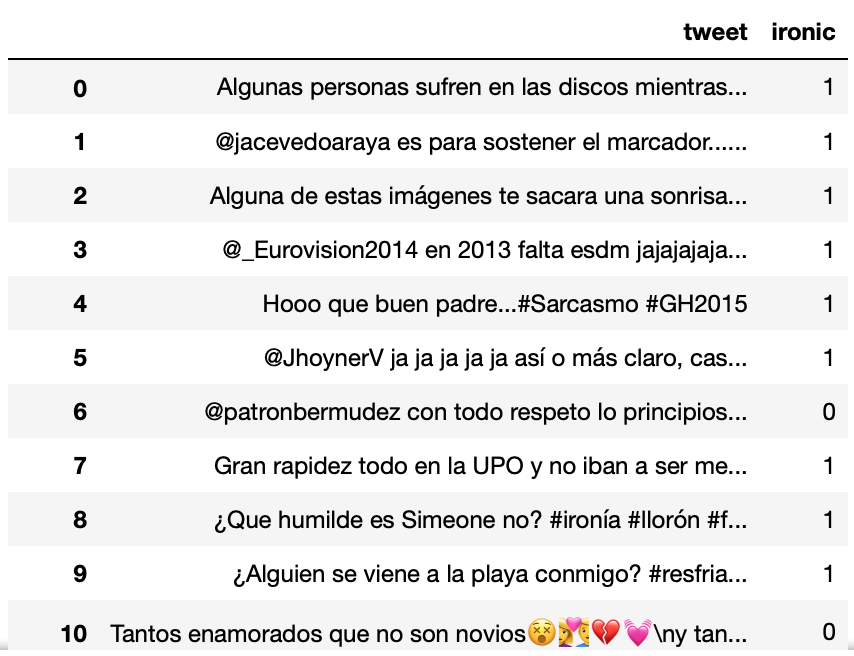
\includegraphics[width=\linewidth]{img/dataset.png}
	\caption{Dataset}
	\label{fig:dataset}
\end{figure}

\section{Preprocessing}
\label{sec:preprocessing}
The preprocessing stage is conceived to dispose of any information that will not be needed during the \ac{ml} step ~\cite{preprocess}. The preprocessing was applied individually to each tweet.
The changes in the dataset that have been made are:
\begin{itemize}
	\item \textit{False items}: Since almost half the dataset tweets come from tweeter, it was required to download those tweets from the social network. Some of the captured tweets were false.
	\item \textit{Categorical values}: Originally the labels of the dataset were either 'True' or 'False'. These two values were encoded into 'True'= 1 and 'False' = 0.
	\item \textit{Stopwords}:  In \ac{ml} it is a very common practice to delete words which barely provide any information to the text (e.g. 'a', 'I', 'you'). In this project, the list of stopwords was chosen for the spanish language due to the language of the tweets. The list of words can be consulted in ~\cite{stopwords}.
	\item \textit{Tokenization}:This process consists of splitting a string (tweet) into tokens. Usually a token is the same as a word.
	\item 
	\textit{Stemming}: This process consists of reducing the tokens into its root. Basically the words are transformed into its root. Stemming was accomplished using a Snowball stemmer. 
\end{itemize}
These steps of preprocessing were all executed defining a custom tokenizer but the categorical value encoding and the false item removal, which were done previously.\\
It is noteworthy to mention that the custom tokenizer is used later for the feature extraction.\\
At the beginning of the preprocessing stage, the dataset is split into two parts, a training part and a testing part. The purpose of this split is to train a clasifier using the train  sequence and evaluate the accuracy of the classifier using the test sequence. The split is taken randomly. The size of each sequence is 75\% for the train sequence and 25\% for the test sequence (8311 and 2771).
\section{Feature Extraction}
 The feature extraction process consist of reading the text and extracting certain features. Furthermore, those extracted features will be fed to the classifier and finally the model will be completed. As a result, the accuracy of the model will be directly related to the choice of features. Therefore, it is very important to choose wisely the features to extract.\\
This section will be committed to extensively explaining the selected features.
\par
The extraction will be performed inside a Pipeline, which will execute each extraction sequentially. In this project, two pipelines are defined, the first aims at extracting the ngrams. With the ngrams extracted from the first pipeline, a second one will extract other features and unify the ngrams with the other extracted features. Even though there are two pipelines defined, the results of the ngrams pipeline are added to the other pipeline. This is done thanks to the Feature Union class provided by Scikit-Learn.
\subsection{Lexical Features}
Usually extracting lexical features involves getting the number of sentences and the number of words in each sentence. However, since this projects' dataset is made out of tweets and the number of characters in a tweet is limited, I have considered that each tweet contains only one sentence. As a consequence, the lexical feature extraction becomes very simple. The extraction consists of tokenizing each sentence and stemming each token (or word) to get the root. At the same time, the words belonging to the spanish stop list are removed (see \cref{sec:preprocessing} for more details). In \todo[inline]{pon aqui la seccion en la que se explica el tfidf} is explained what happens with the extracted words in this stage.
\subsection{Syntactic Features}
\todo[inline]{Esto no aparece en el código}
The syntactic feature extraction consists of counting the number of nouns, adjectives, verbs, adverbs, conjunctions, pronouns and numbers present in each tweet.In \todo[inline]{pon aqui la seccion en la que se explica el tfidf} is explained what happens with the extracted words in this stage.
\subsection{Ngram Features. Pipeline}
Ngram extractions consist of grouping the words into bag of words. If we group the words individually then a sentence with five words will be considered as a five words sentence. If we group two words together then a sentence of six words will be considered as a three word sentence. So each pair of words are understood by the estimator as one.\\
Since it is very difficult to guess what is the optimum bag of words (i.e. number of words) CountVectorizer method provided by the Scikit-Learn class allows us to define a range. Finally, to select the optimum range, a Grid Search will be performed (see \todo[inline]{Pon aqui la seccion donde explicas el grid search}).
\subsection{\ac{lda} Features}
\ac{lda}~\footnote{\url{https://en.wikipedia.org/wiki/Latent_Dirichlet_allocation}} is a generative statistical model that allows sets of observations to be explained by unobserved groups that explain why some parts of the data are similar.\\ In other words, \ac{lda} extraction can be used to extract how many topics are being spoken about in the dataset. This can be observed by analyzing each words' presence.\\
The main parameter of this statistical model is the number of topics. Similarly as with the ngrams features, a Grid Search will be performed to find the optimum number of topics (see \todo[inline]{Pon aqui la seccion donde explicas el grid search}).


